\pdfoutput=1
\documentclass[11pt,a4paper]{article}
\usepackage{abhijit-research}
\renewcommand{\PaperCode}{P07}
\renewcommand{\PaperKind}{RESEARCH PAPER}
\renewcommand{\PaperVersion}{VERSION 1.1}
\renewcommand{\PaperDate}{AUGUST 2026}
\renewcommand{\PaperTitle}{Capacity Complexes}
\renewcommand{\PaperSubtitle}{One-Bit Persistence and Operator-Ideal Criticality}
\renewcommand{\PaperFullTitle}{Capacity Complexes, One-Bit Persistence, and Operator-Ideal Criticality}
\renewcommand{\PaperShortTitle}{Capacity Complexes}
\renewcommand{\PaperKeywords}{capacity complex; persistent homology; squarefree incidence; operator ideals; null transport; scalarization}
\renewcommand{\PaperClassification}{Topological, representation, null-transport, and operator theorems are exact in their displayed source-generated constructions. Classical analytic consequences require the separate bridge in P08.}
\renewcommand{\PaperCitation}{Singh, Abhijit. 2026. \textit{Capacity Complexes, One-Bit Persistence, and Operator-Ideal Criticality}. Research manuscript, version 1.0.}
\begin{document}
\MakeResearchTitle
\MakeResearchContents
\MakeResearchAbstract{%
Binary capacity and prime-transparent coordinates generate a squarefree arithmetic carrier under a shared logarithmic budget. The resulting quota complex admits an explicit acyclic matching: every odd squarefree carrier $m$ produces one reduced homology class with exact persistence interval $[m,2m)$. The signed occupation is the Mertens sum. Retaining all nonbinary resultants gives a standard contrast representation whose full-fibre average cancels the linear charge, producing a quadratic completion boundary. Preservation of generated null pairs independently forces half-cost transport. The orientation operator is Hilbert-Schmidt exactly beyond one half and trace class only beyond one. The uniform odd scalar functional is proved nonclosable on the quadratic carrier. These are exact topological and operator statements, not a proof of a classical zero-location conjecture. Prime-occupation coordinates refine the finite composite sector into squarefree coupling and repeated-prime depth.
}
\section{Binary capacity}
Repeated binary distinction assigns capacity $2^{-r}$ to a depth-$r$ cell. Multiplicativity of independent capacity gives the additive coordinate
\begin{equation}
c(u)=-\log_2u.
\end{equation}
A symmetric $q$-resultant event has ideal capacity $1/q$ per resultant and cost
\begin{equation}
c(q)=\log_2q.
\end{equation}
Independent coordinates therefore satisfy $c(n)=\log_2n$, and the shared budget $c(n)\le\log_2N$ is exactly $n\le N$.

\section{Transparent arities}
Call $q\ge2$ transparent when
\begin{equation}
\binom qk\equiv0\pmod q,\qquad0<k<q.
\end{equation}
\begin{theorem}[Prime transparency]
An arity is transparent if and only if it is prime.
\end{theorem}
\begin{proof}
For prime $q$, divisibility is immediate. If $q$ is composite and $p\mid q$ is prime, then $\binom qp=(q/p)\binom{q-1}{p-1}$ lacks one factor $p$ required for divisibility by $q$.
\end{proof}
This is a classical arithmetic equivalence used here after the cost construction; novelty is not claimed for the equivalence itself.

\section{Squarefree incidence orientation}
Independent prime coordinates yield finite-support exponent vectors and unique factorization. On squarefree support, Boolean incidence inversion gives
\begin{equation}
\mu(n)=(-1)^{\omega(n)},
\end{equation}
with $\mu(n)=0$ when a prime repeats. A continuous character of additive cost is $2^{-sc}$ and becomes $n^{-s}$ on generated integer identities. In the absolute domain,
\begin{equation}
\sum_{n\ge1}\mu(n)n^{-s}=\prod_p(1-p^{-s}).
\end{equation}

\section{Quota complex}
Define
\begin{equation}
K_N=\left\{A\subset\mathbb P:\prod_{p\in A}p\le N\right\}.
\end{equation}
Pair every odd squarefree $m$ with $2m$ whenever $2m\le N$.
\begin{theorem}[Binary capacity homotopy]
The reduced complex is homotopy equivalent to a wedge with one sphere of dimension $\omega(m)-1$ for each odd squarefree $m$ satisfying
\begin{equation}
N/2<m\le N.
\end{equation}
\end{theorem}
The signed Euler occupation is the Mertens sum
\begin{equation}
M(N)=\sum_{n\le N}\mu(n).
\end{equation}

\section{Exact persistence barcode}
Each odd squarefree $m$ births one class at $N=m$ and dies when its binary cone appears at $N=2m$. The complete interval is
\begin{equation}
\boxed{[m,2m),}
\end{equation}
or one bit in logarithmic capacity.

\begin{figure}[H]\centering
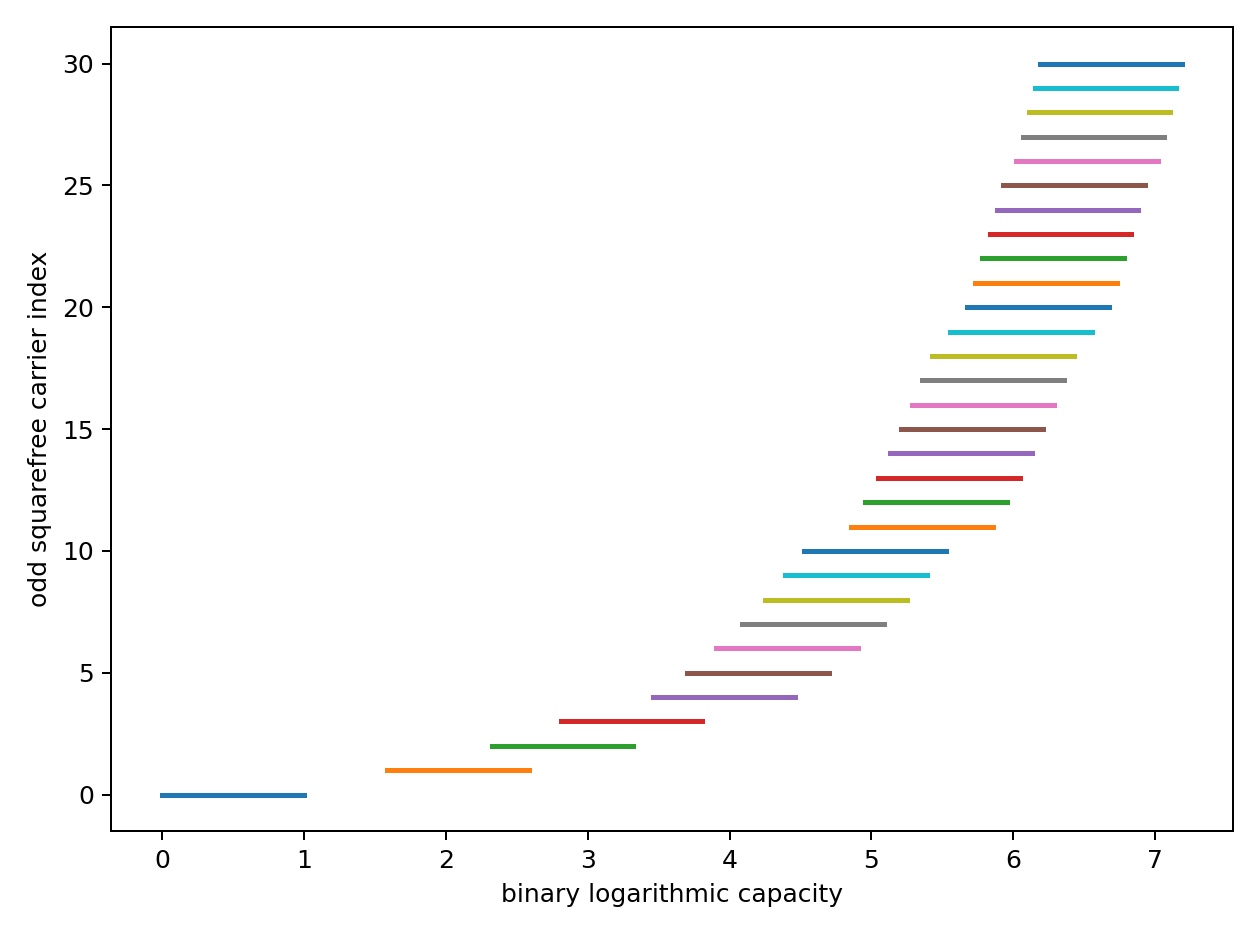
\includegraphics[width=.78\linewidth]{figures/p7_capacity_barcode.png}
\caption{Initial one-bit persistence intervals for odd squarefree carriers.}
\end{figure}

\section{Nonbinary contrast fibres}
A $q$-resultant relation decomposes into one collective direction and the $(q-1)$-dimensional standard contrast representation. The permutation character is
\begin{equation}
\chi_q(\pi)=\#\operatorname{Fix}(\pi)-1.
\end{equation}
Full relabelling-fibre averaging cancels the linear contrast charge; the normalized all-channel determinant begins quadratically and completes in the half-plane $\Re s>1/2$. This is a statement about the uncollapsed contrast response, not by itself about a scalar Dirichlet series.

\section{Null transport and the half exponent}
The generated null pairing is preserved only when local transport satisfies
\begin{equation}
a_p(s)^2=p^s,
\end{equation}
so
\begin{equation}
a_p(s)=\pm p^{s/2}.
\end{equation}
The exponent $1/2$ is therefore forced within the null-preservation law.

\section{Orientation operator}
On the squarefree basis $w_n$, define
\begin{equation}
Jw_n=\mu(n)w_n,\qquad Hw_n=(\log n)w_n,\qquad D_s=Je^{-sH}.
\end{equation}
The singular values are $n^{-\Re s}$ on squarefree carriers.
\begin{theorem}[Operator-ideal thresholds]
$D_s$ is Hilbert-Schmidt exactly for $\Re s>1/2$ and trace class exactly for $\Re s>1$.
\end{theorem}
\begin{proof}
The Hilbert-Schmidt sum is $\sum_{n\text{ sf}}n^{-2\Re s}$, which converges exactly when $2\Re s>1$. The trace-norm sum is $\sum_{n\text{ sf}}n^{-\Re s}$, converging exactly for $\Re s>1$.
\end{proof}

\section{Scalar nonclosability}
Let $S_N$ be the visible squarefree set and
\begin{equation}
X_N=|S_N|^{-1}\sum_{n\in S_N}\mu(n)|n\rangle\langle n|.
\end{equation}
Then $\|X_N\|_2\to0$ while $\Tr(JX_N)=1$.
\begin{theorem}[Odd-trace obstruction]
The uniform signed scalar functional is not closable on the quadratic Hilbert-Schmidt carrier.
\end{theorem}
This proves that the quadratic completion does not automatically supply the desired scalar estimate. It does not prove that every special scalar trajectory diverges.

\section{Clifford orientation charge}
Retaining oriented prime creation yields generators $\gamma_p$ with
\begin{equation}
\gamma_p^2=I,\qquad \gamma_p\gamma_q+\gamma_q\gamma_p=0\quad(p\ne q),\qquad J\gamma_p+\gamma_pJ=0.
\end{equation}
The odd charge
\begin{equation}
\Gamma_P(s)=\sum_{p\in P}p^{-s}\gamma_p
\end{equation}
satisfies
\begin{equation}
\Gamma_P(s)^2=\left(\sum_{p\in P}p^{-2s}\right)I,
\end{equation}
so it has a natural half-cost completion. Sending all $\gamma_p$ to one scalar is not an algebra homomorphism.

\section{Prime-occupation refinement of the composite sector}
The prime/composite split of the finite terminal lattice is too coarse for M\"obius continuation. Introduce occupation labels
\begin{equation}
N_p|d\rangle=v_p(d)|d\rangle,
\qquad p\in\{2,3,5,7\}.
\end{equation}
Then
\begin{equation}
6\leftrightarrow(1,1,0,0)
\end{equation}
is squarefree coupling, whereas
\begin{equation}
4\leftrightarrow(2,0,0,0),\quad8\leftrightarrow(3,0,0,0),\quad9\leftrightarrow(0,2,0,0)
\end{equation}
contain repeated prime coordinates. Accordingly $\mu(6)=+1$ but $\mu(4)=\mu(8)=\mu(9)=0$.

This finite refinement explains why equal prime/composite Fourier magnitudes do not imply M\"obius cancellation. The arithmetic source distinguishes support, orientation, and repeated depth. The 36-cell relation frontier captures all binary differences among nine active indices, but an all-prime continuation requires unbounded finite support addresses rather than a fixed finite label set.

\section{Claim boundary}
The capacity complex, matching, barcode, contrast representation, null-transport exponent, operator thresholds, and scalar nonclosability are exact within the displayed constructions. The appearance of $1/2$ is an operator and geometric boundary. Any identification with a classical critical line requires an additional exact bridge, supplied only in the companion completion paper.


\section{Prime transparency and generated arithmetic}
A symmetric $q$-resultant event assigns cost $\log_2q$. Intermediate capacities are the binomial coefficients. Define transparency by
\begin{equation}
\binom qk\equiv0\pmod q,\qquad0<k<q.
\end{equation}
For prime $q$ divisibility is immediate. If $q$ is composite and $p\mid q$ is prime, then
\begin{equation}
\binom qp=\frac qp\binom{q-1}{p-1}
\end{equation}
lacks the required factor of $p$ for divisibility by $q$. Thus transparent arities are exactly the primes. Independent transparent coordinates generate finite exponent vectors, unique factorization, logarithmic cost, and squarefree incidence orientation
\begin{equation}
\mu(n)=(-1)^{\omega(n)},
\end{equation}
with zero when a coordinate repeats.

\section{Capacity complex and matching proof}
For $N\ge1$ define
\begin{equation}
K_N=\left\{A\subset\mathbb P:\prod_{p\in A}p\le N\right\}.
\end{equation}
Pair every odd squarefree $m$ with $2m$ whenever $2m\le N$. The matching is acyclic because matched edges strictly change membership of the distinguished prime 2 and no alternating cycle can return with the same orientation. Unmatched cells are exactly odd squarefree $m$ with
\begin{equation}
\frac N2<m\le N.
\end{equation}
Discrete Morse reduction therefore gives one sphere of dimension $\omega(m)-1$ for each unmatched $m$. Every class is born at $N=m$ and killed when its binary cone enters at $N=2m$:
\begin{equation}
\boxed{[m,2m)}.
\end{equation}
The interval has width one in logarithmic binary cost. Its signed occupation is the Mertens sum.

\section{Nonbinary contrasts and half-cost transport}
A $q$-resultant relation decomposes into one collective direction and the $(q-1)$-dimensional standard contrast representation. Complete relabelling averages the linear contrast charge to zero, so the normalized determinant begins quadratically. Separately, preservation of the generated null pair requires a local transport amplitude satisfying
\begin{equation}
a_p(s)^2=p^s,
\end{equation}
forcing $a_p(s)=\pm p^{s/2}$. The exponent one half is therefore derived twice in distinct structures: quadratic contrast completion and null preservation. Neither derivation alone supplies a scalar cancellation estimate.

\section{Operator completion and scalarization barrier}
On the squarefree basis $w_n$, set
\begin{equation}
Jw_n=\mu(n)w_n,\qquad Hw_n=(\log n)w_n,\qquad D_s=Je^{-sH}.
\end{equation}
The singular values are $n^{-\Re s}$. Thus $D_s$ is Hilbert--Schmidt exactly for $\Re s>1/2$ and trace class exactly for $\Re s>1$.

The odd scalar is not closable on the quadratic carrier. Let $S_N$ be the visible squarefree set and
\begin{equation}
X_N=|S_N|^{-1}\sum_{n\in S_N}\mu(n)|n\rangle\langle n|.
\end{equation}
Then $\|X_N\|_2=|S_N|^{-1/2}\to0$ while $\Tr(JX_N)=1$. Therefore ordinary scalar trace cannot be extended continuously from finite rank to the half-cost Hilbert--Schmidt completion. The obstruction is exact; it does not prove that every special scalar trajectory diverges.

\section{What this paper contributes}
The topology and operator theory are affirmative results: an exact barcode, an exact operator-ideal boundary, and an exact nonclosability witness. The universal arithmetic cancellation problem begins only after scalarization and is treated in the companion paper rather than smuggled into this one.

\begin{thebibliography}{99}
\bibitem{edelsbrunner} H. Edelsbrunner and J. Harer, Computational Topology, American Mathematical Society, 2010.
\bibitem{forman} R. Forman, Morse theory for cell complexes, Advances in Mathematics 134 (1998), 90--145.
\bibitem{simon} B. Simon, Trace Ideals and Their Applications, American Mathematical Society, 2005.
\bibitem{lawson} H. B. Lawson and M.-L. Michelsohn, Spin Geometry, Princeton University Press, 1989.
\bibitem{titch} E. C. Titchmarsh, revised by D. R. Heath-Brown, The Theory of the Riemann Zeta-Function, Oxford University Press, 1986.
\end{thebibliography}
\end{document}
